\chapter{CRAFTS Architecture}
\label{ch:architecture}
CRAFTS is built to be as simple to deploy and configure as possible. The \texttt{crafts-cli} script provides options for setting up a CRAFTS database within CouchDB, as well as automatically loading all of the view and list functions CRAFTS requires to operate.

Once the database is configured, the CRAFTS daemon, \texttt{craftsd}, can be launched. \texttt{craftsd} is the primary executable for running the CRAFTS service. It takes in the CouchDB URL, name of the database, and the configuration document ID as parameters. The rest of this chapter goes into detail about how CRAFTS can be deployed, how it handles errors, how it can be configured, and how to access its data through the web UI.

\section{Deployment}
In order to make CRAFTS as accommodating of different system configurations and workflows as possible, it supports a number of methods of deployment. Detailed instructions for each method can be found in \Cref{ap:installing}

\subsection{Building from Source}
CRAFTS uses a Python utility called VirtualEnv which packages all of its dependencies, including a Python binary, together with the source code. Running CRAFTS from source is as easy as downloading or cloning the source repository, configuring the database using \texttt{crafts-cli}, and launching the CRAFTS daemon, \texttt{craftsd}.

\subsection{Installing with Pip}
CRAFTS is registered with the Python Package Index (PyPI) and can be installed on any machine running Python 2.7 using \texttt{pip}. Pip is the recommended Python packaging manager and can be used to install packages, their dependencies, as well as set up services.

\subsection{Docker}
Docker is a wrapper around Linux containers, an OS-level virtualization solution for running isolated Linux systems on a single host. Docker is rapidly growing in popularity as a deployment tool due to its ease of use and ability to run on almost any modern Linux based system without the performance overhead of traditional virtual machines.

CRAFTS can be built as a complete docker container. This container includes a pre-configured CouchDB instance and only requires the specification of a configuration file to be loaded into Couch on startup.

\subsection{Vagrant}
Vagrant is a headless virtual machine manager which allows for easy creation and management of development environments. CRAFTS supplies a Vagrantfile for easy creation of a development environment which includes the CRAFTS source code and all necessary dependencies, including a running CouchDB instance.

\section{Command-line Setup Utility}
CRAFTS offers a command-line setup utility called \texttt{crafts-cli}. The utility provides three commands: \texttt{init}, \texttt{update}, and \texttt{clear}. The \texttt{init} command takes CouchDB connection information and a configuration file as parameters and creates a database for CRAFTS in CouchDB. It also automatically creates all of the view and list functions necessary for CRAFTS to run and upload the specified configuration document. Mostly for debugging purposes, the \texttt{update} command re-uploads all of the view and list functions to CouchDB. Finally, the \texttt{clear} command can be used to remove the CRAFTS database from CouchDB.

\section{Configuring CRAFTS}
All of CRAFTS' configuration is pulled from the document specified when \texttt{craftsd} is launched. This means that there can be more than one configuration stored in the database, but one must be chosen at startup. All instances of \texttt{craftsd} should use the same configuration in order to avoid undefined behavior. The following sections discuss some of the more important aspects of configuration. A more detailed explanation of the CRAFTS configuration format and its paramaters can be found in \Cref{ap:craftsconfig}.

\subsection{Choosing Modules}
When \texttt{craftsd} downloads the configuration, it dynamically imports the modules specified in their respective fields. If a module requires its own additional configuration, this information can be stored under a key of the same name in the configuration. This is not a required naming convention because the entire configuration is passed to all modules, but it is a good practice to avoid confusion.

\subsection{Logging}
\texttt{craftsd} supports Python logging configuration files as attachments to the configuration document which will then be read on startup. CRAFTS also offers a special handler for putting log information back into CouchDB called Glitter. Glitter takes Python LogRecord objects and puts all of their attributes into a JSON document for storage in CouchDB. This makes the logs queryable through CouchDB views and easy to monitor remotely. This is especially useful in the event of a fail-over, all \texttt{craftsd} logging data stays contained in CRAFTS' main dependency.

\section{CRAFTS Web UI}
CRAFTS provides a web interface which displays its predictions and scaling plans laid over observed load. This allows engineers a visual method of validating the accuracy of CRAFTS decisions. This interface also includes markers for events such as when a tuning was run, as well as the results of that tuning. The web server is built in Python using the Flask framework and the charts are built using the Highcharts Highstocks Javascript library.

The web server serves as a proxy between the user interface and CouchDB. The server will ensure that the logged-in user has permissions required to view the requested data and to make queries to CouchDB list functions to retrieve the displayed data.

\begin{figure}
\centering
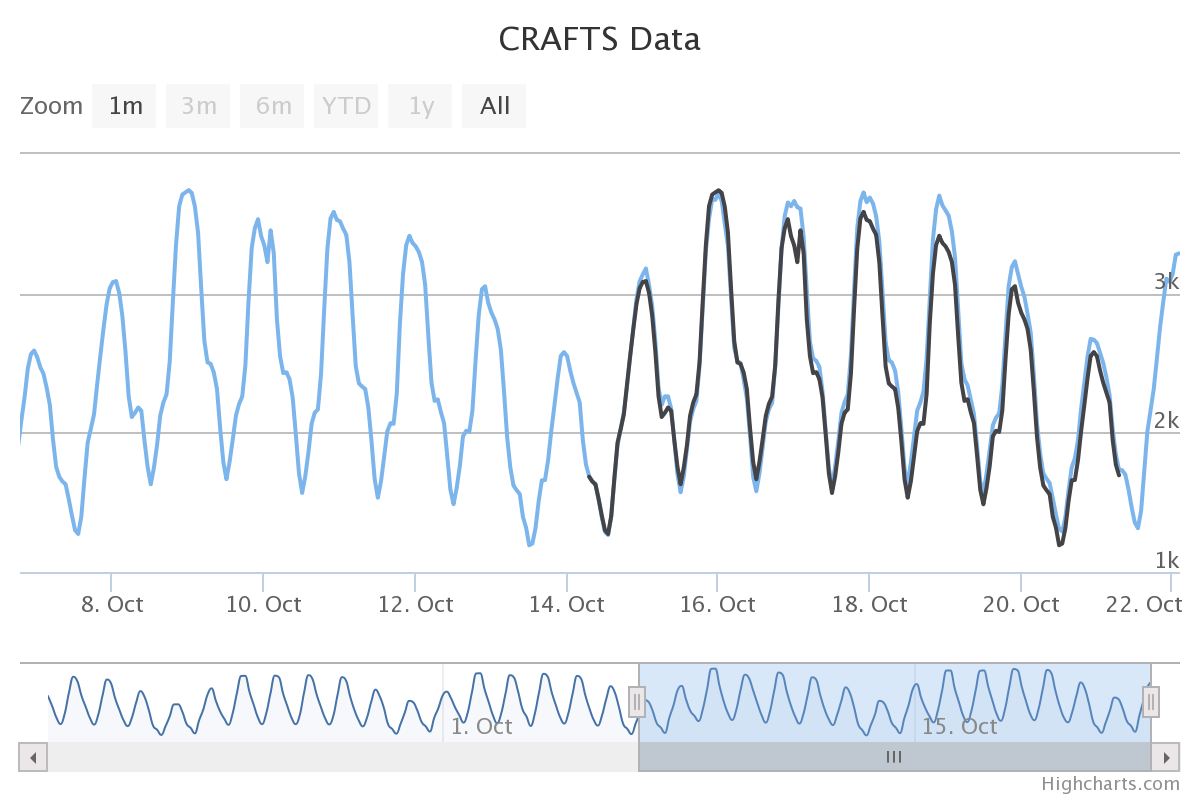
\includegraphics[width=\textwidth]{diagrams/webui.png}
\caption{The CRAFTS web interface}
\label{fig:webui}
\end{figure}